\documentclass[10pt, aspectratio=169]{beamer}

\usetheme[progressbar=frametitle]{metropolis}

\usepackage[utf8]{inputenc}
\usepackage{lmodern}
\usepackage{appendixnumberbeamer}
\usepackage{xcolor}
\usepackage{subcaption}
\usepackage{tikz}
\usepackage{bm}
\usepackage{booktabs}

\usetikzlibrary{arrows,positioning}

\mode<presentation>
% enable the following row to show notes for training your talk
%\setbeameroption{show notes on second screen}


\definecolor{rwthblue}{RGB}{0,84,159}
\definecolor{rwthmagenta}{RGB}{227,0,102}
\definecolor{rwthyellow}{RGB}{255,237,0}
\definecolor{rwthgreen}{RGB}{87,171,39}
\definecolor{rwthred}{RGB}{204,7,30}

\setbeamercolor{normal text}{fg=rwthblue, bg=white}
\setbeamercolor{alerted text}{fg=rwthmagenta}
\setbeamercolor{example text}{fg=rwthyellow}

\newcommand{\source}[1]{
  \begin{tikzpicture}[remember picture, overlay]
    \node[xshift=0cm, yshift=-.3cm, above=of current page.south] {\footnotesize Source: #1};
  \end{tikzpicture}
}

\title{Long Short-Term Memory}
\subtitle{Joint Proseminar on Machine Learning and Image Processing}
\date{February 30, 1337}
\author{Fynn Jansen, Leon Benzer}
\institute{Chair of Computer Science 13 (Computer Vision)\\RWTH Aachen}
\makeatletter
\setbeamertemplate{frame footer}{Long Short-Term Memory \hfill Fynn Jansen, Leon Benz, RWTH}
\makeatother

\begin{document}

\maketitle

% ----------------------------------------------------------------

% Constant Error Carousel
\begin{frame}[t]{Naive Approach - Constant Error Flow}
    Single Unit Constant Error Carousel:
\end{frame}

\begin{frame}[t]{Naive Approach - Constant Error Flow}
    Single Unit Constant Error Carousel:
    \begin{itemize}
        \item Linear activation function : \begin{math}f(x)=x\end{math}
    \end{itemize}
\end{frame}

\begin{frame}[t]{Naive Approach - Constant Error Flow}
    Single Unit Constant Error Carousel:
    \begin{itemize}
        \item Linear activation function : \begin{math}f(x)=x\end{math}
        \item Feedback connection weight : \begin{math}w=1\end{math}
    \end{itemize}
\end{frame}

\begin{frame}[t]{Naive Approach - Constant Error Flow}
    Single Unit (\begin{math}j\end{math}) Constant Error Carousel:
    \begin{itemize}
        \item Linear activation function : \begin{math}f(x)=x\end{math}
        \item Feedback connection weight : \begin{math}w_{jj}=1\end{math}
    \end{itemize}
    \begin{figure}
        \centering
        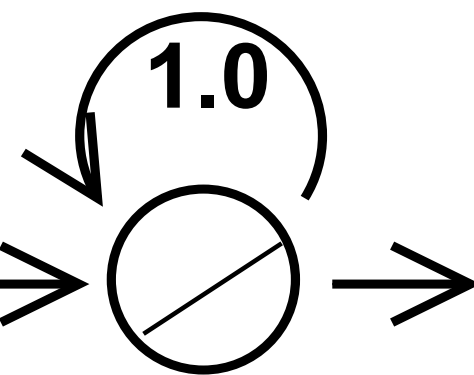
\includegraphics[width=0.25\linewidth]{images/ConstantErrorCarousel.png}
    \end{figure}
\end{frame}

\begin{frame}[t]{Naive Approach - Problems}
\begin{figure}
        \centering
        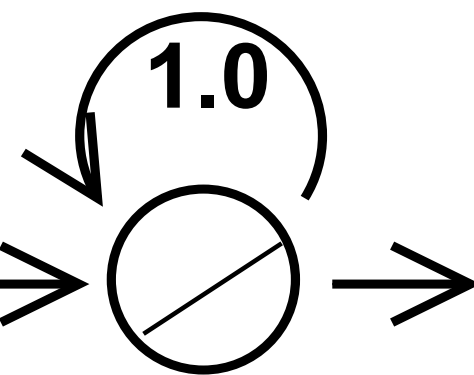
\includegraphics[width=0.25\linewidth]{images/ConstantErrorCarousel.png}
    \end{figure}   
\end{frame}

\begin{frame}[t]{Naive Approach - Problems}
\begin{figure}
        \centering
        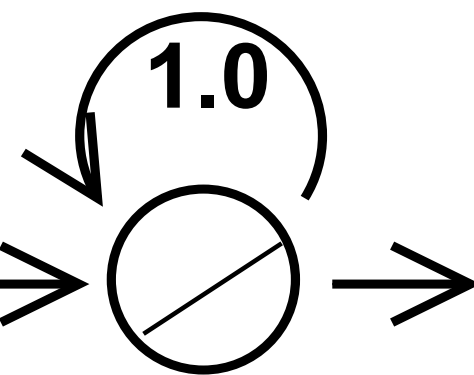
\includegraphics[width=0.25\linewidth]{images/ConstantErrorCarousel.png}
    \end{figure}
Connected to other units:
\end{frame}

\begin{frame}[t]{Naive Approach - Problems}
\begin{figure}
        \centering
        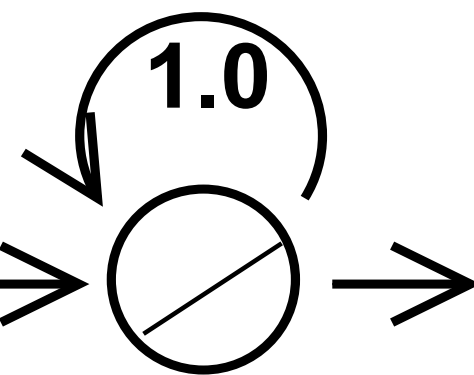
\includegraphics[width=0.25\linewidth]{images/ConstantErrorCarousel.png}
    \end{figure}
Connected to other units:
\begin{itemize}
    \item Input from unit \begin{math}i\end{math}
\end{itemize}
\end{frame}

\begin{frame}[t]{Naive Approach - Problems}
\begin{figure}
        \centering
        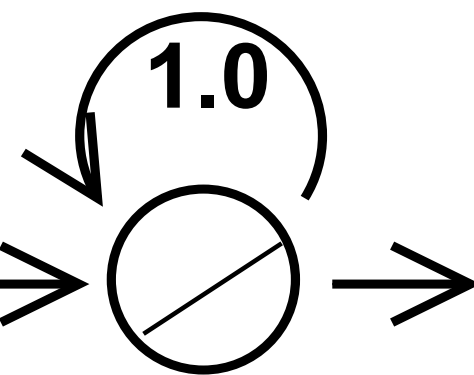
\includegraphics[width=0.25\linewidth]{images/ConstantErrorCarousel.png}
    \end{figure}
Connected to other units:
\begin{itemize}
    \item Input from unit \begin{math}i\implies\end{math}  Single weight \begin{math}w_ji\end{math} for storing \& ignoring inputs
\end{itemize}
\end{frame}

\begin{frame}[t]{Naive Approach - Problems}
\begin{figure}
        \centering
        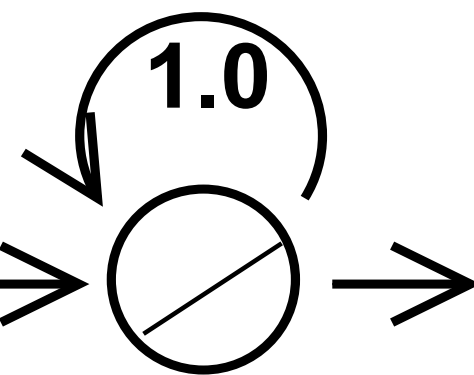
\includegraphics[width=0.25\linewidth]{images/ConstantErrorCarousel.png}
    \end{figure}
Connected to other units:
\begin{itemize}
    \item Input from unit \begin{math}i\implies\end{math} Single weight \begin{math}w_ji\end{math} for storing \& ignoring inputs
    \item Output to unit \begin{math}k\end{math}
\end{itemize}
\end{frame}

\begin{frame}[t]{Naive Approach - Problems}
\begin{figure}
        \centering
        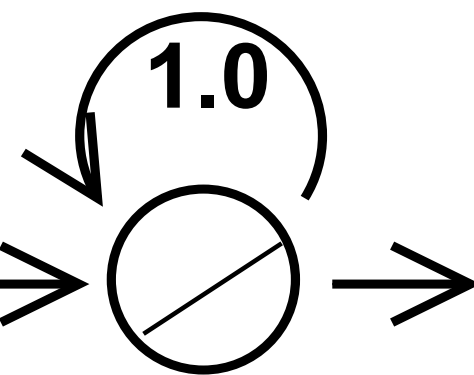
\includegraphics[width=0.25\linewidth]{images/ConstantErrorCarousel.png}
    \end{figure}
Connected to other units:
\begin{itemize}
    \item Input from unit \begin{math}i\implies\end{math} Single weight \begin{math}w_{ji}\end{math} for storing \& ignoring inputs
    
    \item Output to unit \begin{math}k\implies\end{math} Single weight \begin{math}w_{kj}\end{math} for controlling retrieval
\end{itemize}
\end{frame}

\begin{frame}[t]{Naive Approach - Problems}
\begin{figure}
        \centering
        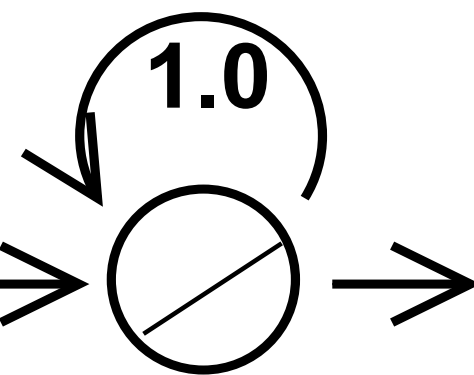
\includegraphics[width=0.25\linewidth]{images/ConstantErrorCarousel.png}
    \end{figure}
Connected to other units:
\begin{itemize}
    \item Input from unit \begin{math}i\implies\end{math} Single weight \begin{math}w_{ji}\end{math} for storing \& ignoring inputs
    
    \item Output to unit \begin{math}k\implies\end{math} Single weight \begin{math}w_{kj}\end{math} for controlling retrieval
\end{itemize}
Conflicting weight update signals for \begin{math}w_{ji}\end{math} \& \begin{math}w_{kj}\end{math}
\end{frame}

\begin{frame}[t]{Naive Approach - Problems}
\begin{figure}
        \centering
        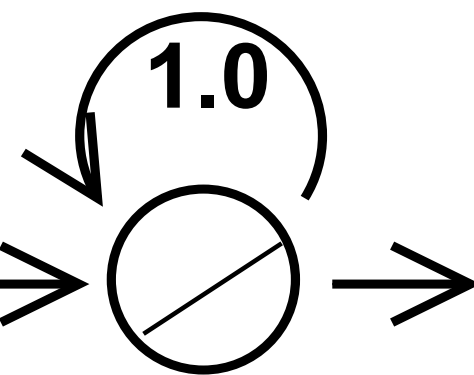
\includegraphics[width=0.25\linewidth]{images/ConstantErrorCarousel.png}
    \end{figure}
Connected to other units:
\begin{itemize}
    \item Input from unit \begin{math}i\implies\end{math} Single weight \begin{math}w_{ji}\end{math} for storing \& ignoring inputs
    
    \item Output to unit \begin{math}k\implies\end{math} Single weight \begin{math}w_{kj}\end{math} for controlling retrieval
\end{itemize}
Conflicting weight update signals for \begin{math}w_{ji}\end{math} \& \begin{math}w_{kj}\implies\end{math} Mechanism for storage and retrieval
\end{frame}

% LSTM Architecture
\begin{frame}[t]{LSTM Architecture - Gate Unit}
Idea: Restrict flow based on context
\end{frame}

\begin{frame}[t]{LSTM Architecture - Gate Unit}
Idea: Restrict flow based on context
\begin{figure}
    \centering
    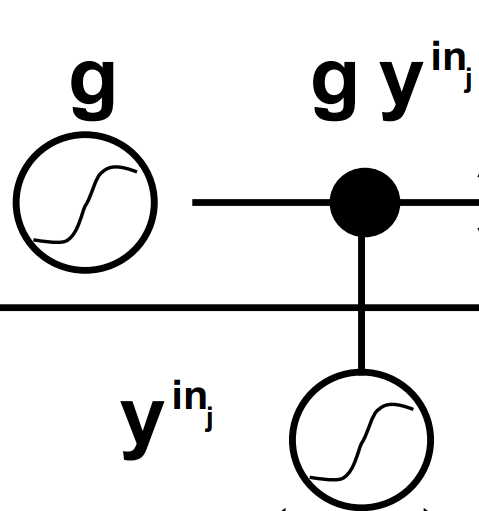
\includegraphics[width=0.2\linewidth]{images/GateUnit.png}
\end{figure}
\end{frame}

\begin{frame}[t]{LSTM Architecture - Gate Unit}
Idea: Restrict flow based on context
\begin{figure}
    \centering
    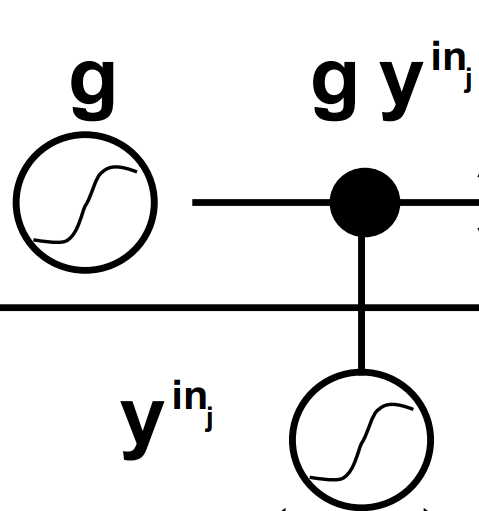
\includegraphics[width=0.2\linewidth]{images/GateUnit.png}
\end{figure}
Input gets scaled by number computed from context
\end{frame}


% LSTM Architecture
\begin{frame}[t]{LSTM Architecture - Memory Cell}
Memory Cell: CEC unit with input and output gate units
\end{frame}

\begin{frame}[t]{LSTM Architecture - Memory Cell}
Memory Cell: CEC unit with input and output gate units
\begin{figure}
    \centering
    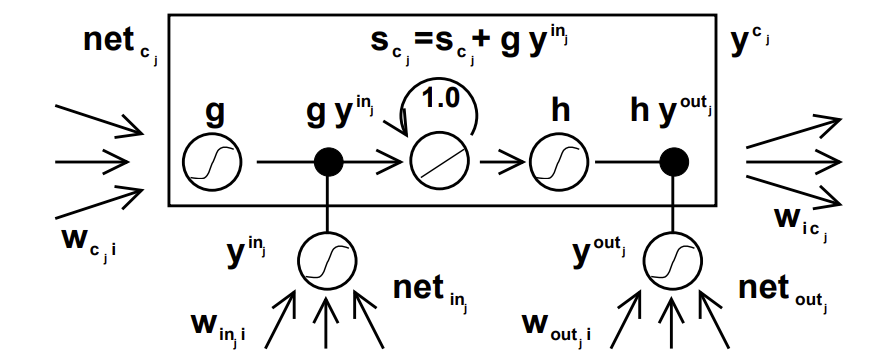
\includegraphics[width=1\linewidth]{images/LSTM-Cell-Diagram.png}
\end{figure}
\end{frame}

\begin{frame}[t]{LSTM Architecture - Network Topology}
Inputs for cell and gates can be chosen:
\end{frame}

\begin{frame}[t]{LSTM Architecture - Network Topology}
Input for cell and gate units can be:
\begin{itemize}
    \item Input Units
\end{itemize}
\end{frame}

\begin{frame}[t]{LSTM Architecture - Network Topology}
Input for cell and gate units can be:
\begin{itemize}
    \item Input Units
    \item Gate Units
\end{itemize}
\end{frame}

\begin{frame}[t]{LSTM Architecture - Network Topology}
Input for cell and gate units can be:
\begin{itemize}
    \item Input Units
    \item Gate Units
    \item Memory Cells
\end{itemize}
\end{frame}

\begin{frame}[t]{LSTM Architecture - Network Topology}
Input for cell and gate units can be:
\begin{itemize}
    \item Input Units
    \item Gate Units
    \item Memory Cells
    \item Conventional Hidden Units
\end{itemize}
\end{frame}

\begin{frame}[t]{LSTM Architecture - Network Topology}
Input for cell and gate units can be:
\begin{itemize}
    \item Input Units
    \item Gate Units
    \item Memory Cells
    \item Conventional Hidden Units
\end{itemize}
Commonly used topology: Inputs for Cell \& Gate are all input units \& memory cell outputs
\end{frame}

\begin{frame}[t]{LSTM Architecture - Network Topology}
Input for cell and gate units can be:
\begin{itemize}
    \item Input Units
    \item Gate Units
    \item Memory Cells
    \item Conventional Hidden Units
\end{itemize}
Commonly used topology: Inputs for Cell \& Gate are all input units \& memory cell outputs
Input Gate: \begin{math}i_t=\sigma_i\left(W_{i\ h}h_{t-1}+W_{i\ x} x_t\right)\end{math}
\end{frame}

\begin{frame}[t]{LSTM Architecture - Network Topology}
Input for cell and gate units can be:
\begin{itemize}
    \item Input Units
    \item Gate Units
    \item Memory Cells
    \item Conventional Hidden Units
\end{itemize}
Commonly used topology: Inputs for Cell \& Gate are all input units \& memory cell outputs
Input Gate:  \begin{math}i_t=\sigma_i\left(W_{i\ h}h_{t-1}+W_{i\ x} x_t\right)\end{math}\\
Output Gate: \begin{math}o_t=\sigma_o\left(W_{o\ h}h_{t-1}+W_{o\ x}x_t\right)\end{math}
\end{frame}

\begin{frame}[t]{LSTM Architecture - Network Topology}
Input for cell and gate units can be:
\begin{itemize}
    \item Input Units
    \item Gate Units
    \item Memory Cells
    \item Conventional Hidden Units
\end{itemize}
Commonly used topology: Inputs for Cell \& Gate are all input units \& memory cell outputs
Input Gate:  \begin{math}i_t=\sigma_i\left(W_{i\ h}h_{t-1}+W_{i\ x} x_t + b_i\right)\end{math}\\
Output Gate: \begin{math}o_t=\sigma_o\left(W_{o\ h}h_{t-1}+W_{o\ x}x_t + b_o\right)\end{math}\\
Cell State: \begin{math}C_t=C_{t-1}+i_t\odot\sigma_c\left(W_{c\ h}h_{t-1}+W_{c\ x}x_t + b_c\right)\end{math} 
\end{frame}

\begin{frame}[t]{LSTM Architecture - Network Topology}
Input for cell and gate units can be:
\begin{itemize}
    \item Input Units
    \item Gate Units
    \item Memory Cells
    \item Conventional Hidden Units
\end{itemize}
Commonly used topology: Inputs for Cell \& Gate are all input units \& memory cell outputs
Input Gate:  \begin{math}i_t=\sigma_i\left(U_{i}h_{t-1}+W_{i} x_t + b_i\right)\end{math}\\
Output Gate: \begin{math}o_t=\sigma_o\left(U_{o}h_{t-1}+W_{o}x_t + b_o\right)\end{math}\\
Internal State: \begin{math}C_t=C_{t-1}+i_t\odot\sigma_c\left(U_{c}h_{t-1}+W_{x}x_t + b_c\right)\end{math}\\
Output: \begin{math}h_t=o_t\odot\sigma_h\left(C_t\right)\end{math}
\end{frame}


\begin{frame}[t]{LSTM Architecture - Limitations}
Drawbacks:
\end{frame}

\begin{frame}[t]{LSTM Architecture - Limitations}
Drawbacks:
\begin{itemize}
    \item Exploding Gradients: Additional methods like gradient clipping needed
\end{itemize}
\end{frame}

\begin{frame}[t]{LSTM Architecture - Limitations}
Drawbacks:
\begin{itemize}
    \item Exploding Gradients: Additional methods like gradient clipping needed
    \item Computational Intensity: Up to 9 times more weights compared to traditional RNN
\end{itemize}
\end{frame}

\begin{frame}[t]{LSTM Architecture - Limitations}
Drawbacks:
\begin{itemize}
    \item Exploding Gradients
    \item Computational Intensity
    \item Limited GPU utilization
\end{itemize}
\end{frame}

\begin{frame}[t]{LSTM Architecture - Limitations}
Drawbacks:
\begin{itemize}
    \item Exploding Gradients
    \item Computational Intensity
    \item Limited GPU utilization
    \item Memory bottlenecks
\end{itemize}
\end{frame}

\begin{frame}[t]{LSTM Architecture - Limitations}
Drawbacks:
\begin{itemize}
    \item Exploding Gradients
    \item Computational Intensity
    \item Limited GPU utilization
    \item Memory bottlenecks
    \item Worse Performance on Short Sequences
\end{itemize}
\end{frame}

\begin{frame}[t]{LSTM Architecture - Limitations}
Drawbacks:
\begin{itemize}
    \item Exploding Gradients
    \item Computational Intensity
    \item Limited GPU Utilization
    \item Memory Bottlenecks
    \item Worse performance on short sequences
    \item State can not be reset
\end{itemize}
\end{frame}


% LSTM Variants
\begin{frame}[t]{Variants - LSTM with forget gate}
Forget Gate:
\end{frame}

\begin{frame}[t]{Variants - LSTM with forget gate}
Forget Gate:
\begin{itemize}
    \item "Forgetting" by resetting state
\end{itemize}
\end{frame}

\begin{frame}[t]{Variants - LSTM with forget gate}
Forget Gate:
\begin{itemize}
    \item "Forgetting" by resetting state
    \item Achieved by gating the previous state
\end{itemize}
\end{frame}

\begin{frame}[t]{Variants - LSTM with forget gate}
Forget Gate:
\begin{itemize}
    \item "Forgetting" by resetting state
    \item Achieved by gating the previous state
    \item \begin{math}f_t=\sigma_i\left(U_{f}h_{t-1}+W_{f} x_t + b_f\right)\end{math}
\end{itemize}
\end{frame}

\begin{frame}[t]{Variants - LSTM with forget gate}
Forget Gate:
\begin{itemize}
    \item "Forgetting" by resetting state
    \item Achieved by gating the previous state
    \item \begin{math}f_t=\sigma_i\left(U_{f}h_{t-1}+W_{f} x_t + b_f\right)\end{math}
    \item \begin{math}C_t=f_t\odot C_{t-1}+i_t\odot\sigma_c\left(U_{c}h_{t-1}+W_{x}x_t + b_c\right)\end{math}
\end{itemize}
\end{frame}

\begin{frame}[t]{Variants - LSTM with forget gate}
\begin{figure}
    \centering
    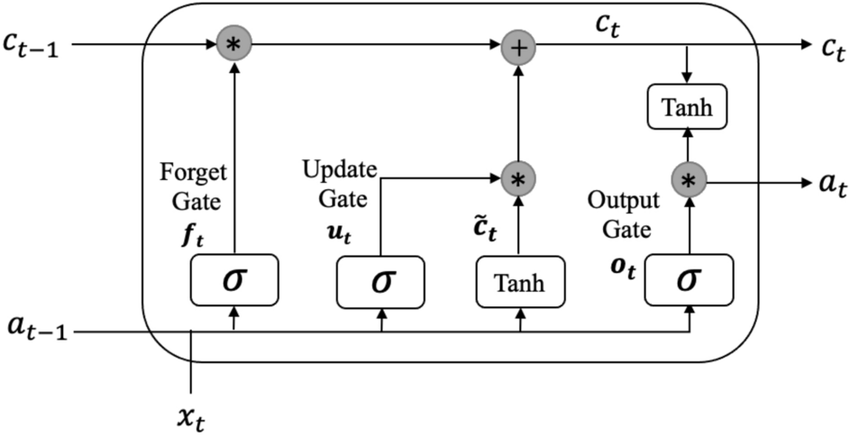
\includegraphics[width=0.75\linewidth]{images/Structure-of-LSTM-cell-which-introduces-three-special-gates-Input-Gate-i-Forget-Gate.png}
\end{figure}
\end{frame}


% ----------------------------------------------------------------
\nocite{DoesNotExist}

\setbeamerfont{bibliography item}{size=\footnotesize}
\setbeamerfont{bibliography entry author}{size=\footnotesize}
\setbeamerfont{bibliography entry title}{size=\footnotesize}
\setbeamerfont{bibliography entry location}{size=\footnotesize}
\setbeamerfont{bibliography entry note}{size=\footnotesize}
\begin{frame}[allowframebreaks]{References}

  \bibliographystyle{alpha}
  \bibliography{slides}

\end{frame}
\end{document}
